\chapter{Einleitung}

Mit Qualitäts-Analysetools, wie z.B. SonarQube\footcite{sonarqube}, können ganze Softwaresysteme kontinuierlichen Qualitätstests unterzogen werden.
Durch die ermittelten Kennzahlen können Aussagen zur Qualität des gesamten Systems, über einzelne Komponenten, bis hin zu einer einzelnen Quellcode-Datei getroffen werden.

Auch Scrum\footcite{scrum} wird als agiles Vorgehensmodell in der Softwareentwicklung immer beliebter. 
Dabei wird bei mehreren Teams, die auf vielen Systeme arbeiten, auf 2 Arten von Scrum Teams zurückgegriffen:
Feature- oder Komponenten-Teams.

Feature-Teams bieten dabei den Vorteil, näher am Scrum Workflow zu sein, da alle Arbeiten an einem Feature von einem Team erledigt werden. Damit das möglich ist, braucht es aber ein breites Wissen über alle Plattformen innerhalb des Teams.
Komponenten-Teams sind im Gegensatz dazu nur für bestimmte Komponenten in einzelnen Plattformen verantwortlich, dafür kann eine Feature-Umsetzung aber mehrere Sprints dauern und es muss bei der Planung auf Abhängigkeiten geachtet werden.

\begin{savenotes}
  \begin{figure}[H] 
    \centering
       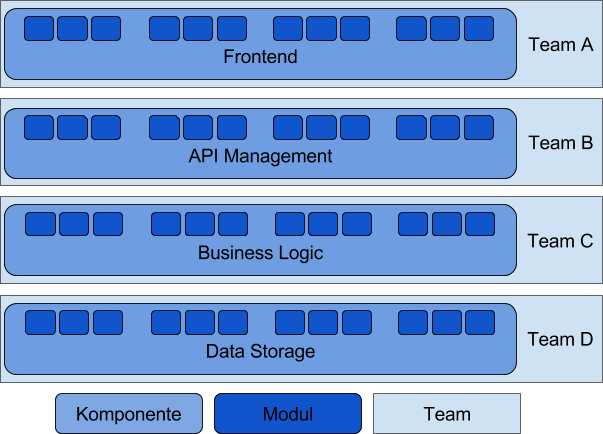
\includegraphics[width=0.7\textwidth]{img/component-teams.png}
    \caption[Komponenten Teams in Scrum]{Komponenten Teams in Scrum}\label{fig:Komponenten Teams in Scrum}
  \end{figure}
\end{savenotes}

Diese Arbeit beschäftigt sich mit Komponenten-Teams und damit verbunden einem komponentenbasierten Qualitätsmanagement auf teamübergreifenden Plattformen.
Das bedeutet, dass Kennzahlen zu Qualitätsmerkmalen nicht auf System-, sondern auf Komponentenebene gesammelt und aggregiert werden, um für jedes Team eine individuelle Sicht auf das Qualitätsmanagement zu ermöglichen.
Um das zu ermöglichen, wird erst eine Vorgehensweise zur Ermittlung von relevanten Kennzahlen entwickelt und diese an einer Beispiel-Organisation angewendet.
Zur Sammlung, Auswertung und Darstellung dieser Kennzahlen wird eine Software entwickelt, die in eine bestehende Umgebung integriert werden kann.
